\documentclass[12pt]{article}
\usepackage{graphicx}
\usepackage{subcaption}
\usepackage{float}
\usepackage{hyperref}

\title{EE236: Experiment 8\\
I-V Characteristics of Solar Cell}

\author{Aaron John Sabu, 170070050}

\begin{document}
\maketitle

\section{Aim of the experiment}

The experiment is meant for the student to realise the curve taken by the current across a solar cell as the voltage across it is varied. Moreover the student understand how exactly the solar cell can act as a source in the fourth quadrant.

\section{Methods}

The experiment was performed using a solar cell box marked with the number 04. This box comprised of a solar cell and an LED bank consisting of 24 white LEDs. The voltmeter and ammeters were provided via the two portable Digital Multimeters and the provided one as well. As a common method for all three steps, the LEDs in the box were lighted using a voltage supply which was connected to the ammeter.

\subsection{Part 1}

The voltage source was connected to a buffer/unity-gain amplifier whose output was connected to a 100 \(\Omega\) resistor which in turn was connected to the ammeter. The ammeter was connected to the n-terminal of the solar cell, whereas the p-terminal was connected to ground and the voltage across the solar cell was measured using a voltmeter.


\begin{figure}[H]
	\centering
	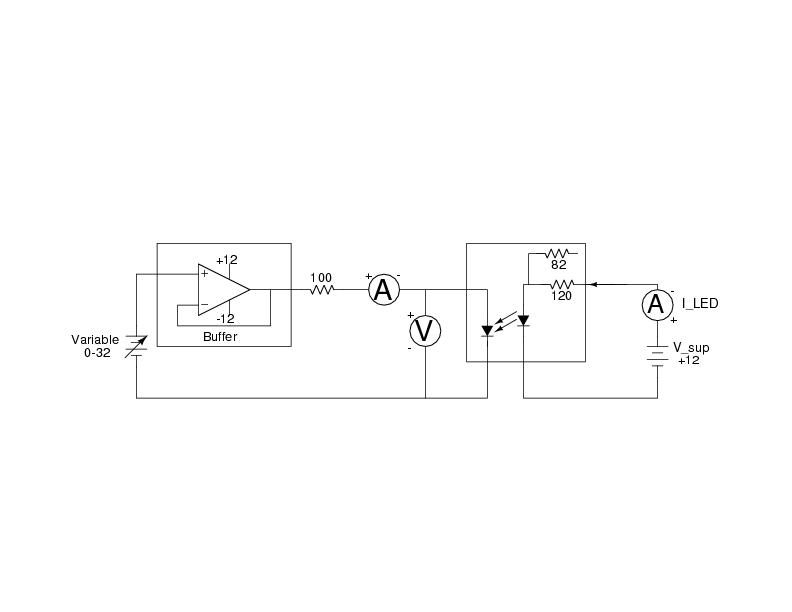
\includegraphics[width = 1.1\linewidth, trim = {0 7cm 2.5cm 6cm}, clip]{Part1_CD.png}
	\caption{Part 1 Circuit Diagram}
\end{figure}

\subsection{Part 2}

Two potentiometers, one of 500\(\Omega\) and one of 100\(\Omega\) were used in series. These were in turn connected to an ammeter. The ammeter and the voltmeter served the same purpose as in part 1.

\begin{figure}[H]
	\centering
	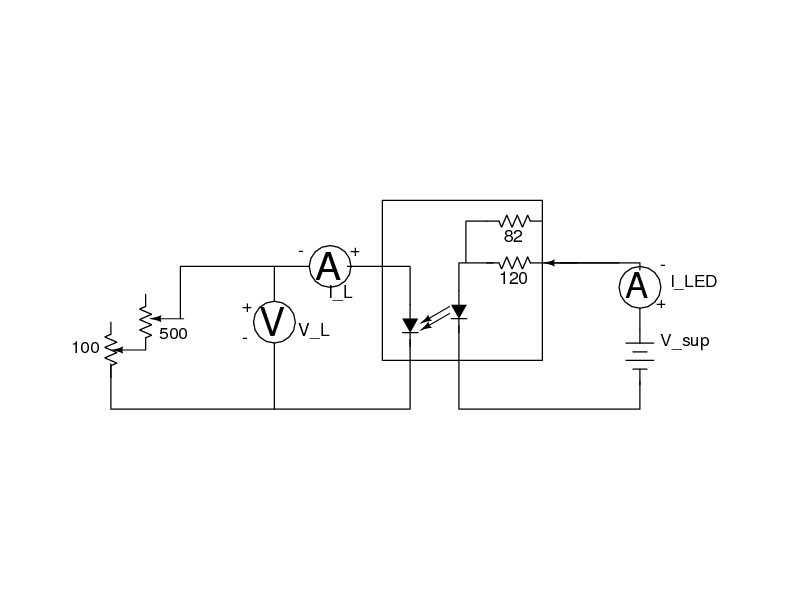
\includegraphics[width = 0.8\linewidth, trim = {2cm 7cm 2.5cm 7cm}, clip]{Part2_CD.png}
	\caption{Part 2 Circuit Diagram}
\end{figure}

\subsection{Part 3}

The ammeter and voltmeter were directly and independently connected to the solar cell, with the purpose of measuring the short circuit current (\(I_{SC}\)) and the open circuit voltage (\(V_{OC}\)) respectively.

\begin{figure}[H]
	\centering
	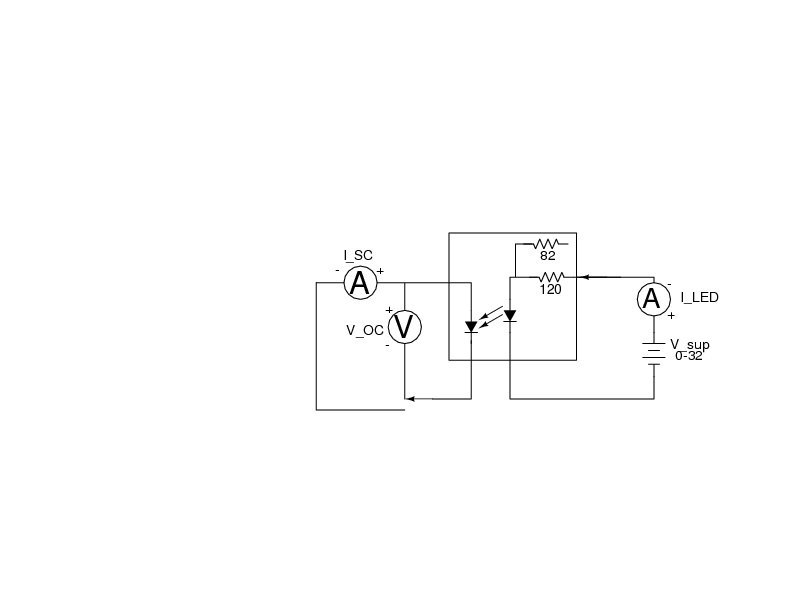
\includegraphics[width = 0.8\linewidth, trim = {7cm 6.5cm 2.5cm 8cm}, clip]{Part3_CD.png}
	\caption{Part 3 Circuit Diagram}
\end{figure}

\section{Observations}

The experiment was conducted in room temperature at approximately sea level atmospheric pressure. Due to these factors, the solar cell was expected to provide sensible results. Here are the results we obtained:

\subsection{Part 1}

We obtained the readings of current flowing through the solar panel and voltage across the solar panel as mentioned in the table and plotted current vs voltage.

\begin{figure}[H]
	\centering
	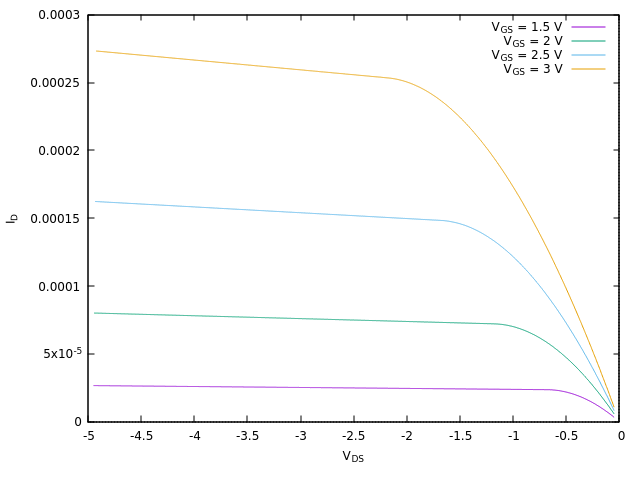
\includegraphics[width = \linewidth, trim = {0 0 0 0}, clip]{Part1.png}
	\caption{Part 1 - I-V Characteristics}
\end{figure}

\begin{center}
 \begin{tabular}{|| c c | c c | c c ||} 
 \hline
 \multicolumn{2}{||c|}{Dark} & \multicolumn{2}{c|}{I1} & \multicolumn{2}{c||}{I2}\\
 \hline
 \hline
 \( V_{SOLAR} (V) \) & \( I_{SOLAR} (mA) \) & \( V_{SOLAR} (V) \) & \( I_{SOLAR} (mA) \) & \( V_{SOLAR} (V) \) & \( I_{SOLAR} (mA) \) \\ [0.25ex] 
 \hline\hline
 \hline 
-1.952 & -0.45 & -1.082 & -9.07 & -0.547 & -11.82 \\ \hline
-1.754 & -0.41 & -0.697 & -8.99 & -0.327 & -11.78 \\ \hline
-1.592 & -0.37 & -0.482 & -8.94 & -0.217 & -11.77 \\ \hline
-1.402 & -0.32 & -0.267 & -8.90 & -0.081 & -11.75 \\ \hline
-1.147 & -0.26 & -0.043 & -8.85 & -0.007 & -11.74 \\ \hline
-0.920 & -0.21 & 0.009 & -8.84 & 0.019 & -11.85 \\ \hline
-0.794 & -0.18 & 0.121 & -8.80 & 0.059 & -11.84 \\ \hline
-0.557 & -0.13 & 0.191 & -8.73 & 0.117 & -11.81 \\ \hline
-0.364 & -0.08 & 0.240 & -8.61 & 0.289 & -11.36 \\ \hline
-0.165 & -0.04 & 0.279 & -8.45 & 0.338 & -10.83 \\ \hline
-0.099 & -0.02 & 0.334 & -7.97 & 0.375 & -10.03 \\ \hline
0.075 & 0.02 & 0.359 & -7.48 & 0.387 & -9.63 \\ \hline
0.230 & 0.20 & 0.387 & -6.72 & 0.404 & -8.90 \\ \hline
0.400 & 2.28 & 0.403 & -6.10 & 0.421 & -8.00 \\ \hline
0.445 & 4.59 & 0.411 & -5.67 & 0.433 & -7.15 \\ \hline
0.461 & 5.89 & 0.423 & -5.05 & 0.442 & -6.28 \\ \hline
0.483 & 8.25 & 0.432 & -4.45 & 0.449 & -5.60 \\ \hline
0.496 & 10.21 & 0.451 & -3.08 & 0.455 & -4.90 \\ \hline
0.508 & 12.22 & 0.456 & -2.42 & 0.464 & -3.60 \\ \hline
0.516 & 14.20 & 0.461 & -1.90 & 0.467 & -3.40 \\ \hline
0.529 & 17.30 & 0.467 & -1.18 & 0.473 & -2.59 \\ \hline
0.537 & 19.70 & 0.471 & -0.65 & 0.481 & -1.24 \\ \hline
0.545 & 20.50 & 0.474 & -0.18 & 0.486 & -0.28 \\ \hline
0.552 & 22.40 & 0.475 & -0.03 & 0.487 & -0.11 \\ \hline
- & - & 0.476 & 0.16 & 0.488 & 0.06 \\ \hline
- & - & 0.480 & 0.69 & 0.489 & 0.17 \\ \hline
- & - & 0.483 & 1.22 & 0.492 & 0.74 \\ \hline
- & - & 0.488 & 2.04 & 0.496 & 1.65 \\ \hline
- & - & 0.496 & 3.35 & 0.504 & 3.26 \\ \hline
- & - & 0.511 & 6.41 & 0.517 & 6.48 \\ \hline
- & - & 0.522 & 8.93 & 0.528 & 9.28 \\ \hline
\end{tabular}
\end{center}

\subsection{Part 2}

Given below are the values obtained for the voltage across the resistance \( V_L \), the current flowing through them \( I_L \) and the the power provided \( P_L = V_L \times I_L \).\\
For illumination current I1, we obtained: \[ I_{LED} = I_{LED_{I1, 12V}} = 0.03 mA\] \[I_{SC} = 8.80 mA\] \[V_{OC} = 0.474 V\] and for illumination current I2, we obtained: \[ I_{LED} = I_{LED_{I2, 12V}} = 0.04 mA\] \[I_{SC} = 11.69 mA\] \[V_{OC} = 0.485 V\]

\begin{figure}[H]
	\begin{subfigure}[b]{0.6\linewidth}
	   	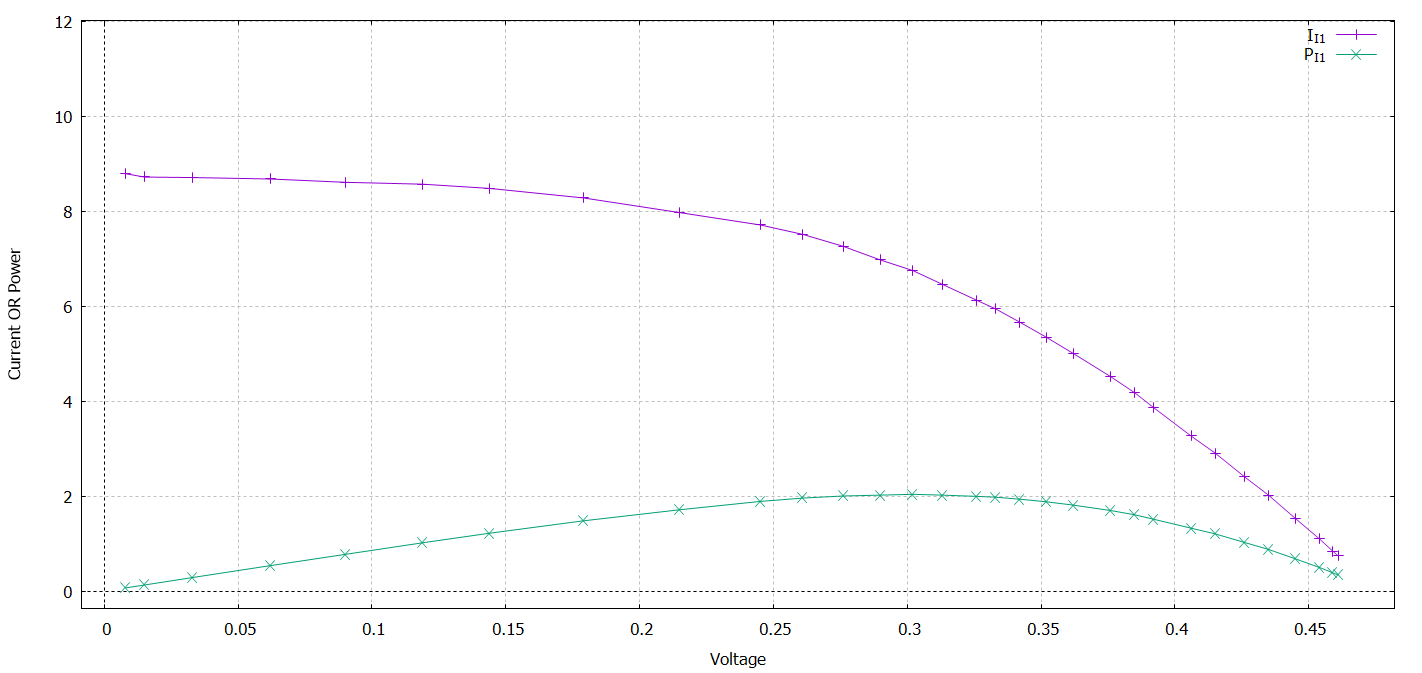
\includegraphics[width = \linewidth, trim = {0 0 0 0}, clip]{Part2_I1.png}
		\caption{Illumination Current I1}
	\end{subfigure}
	\begin{subfigure}[b]{0.6\linewidth}
		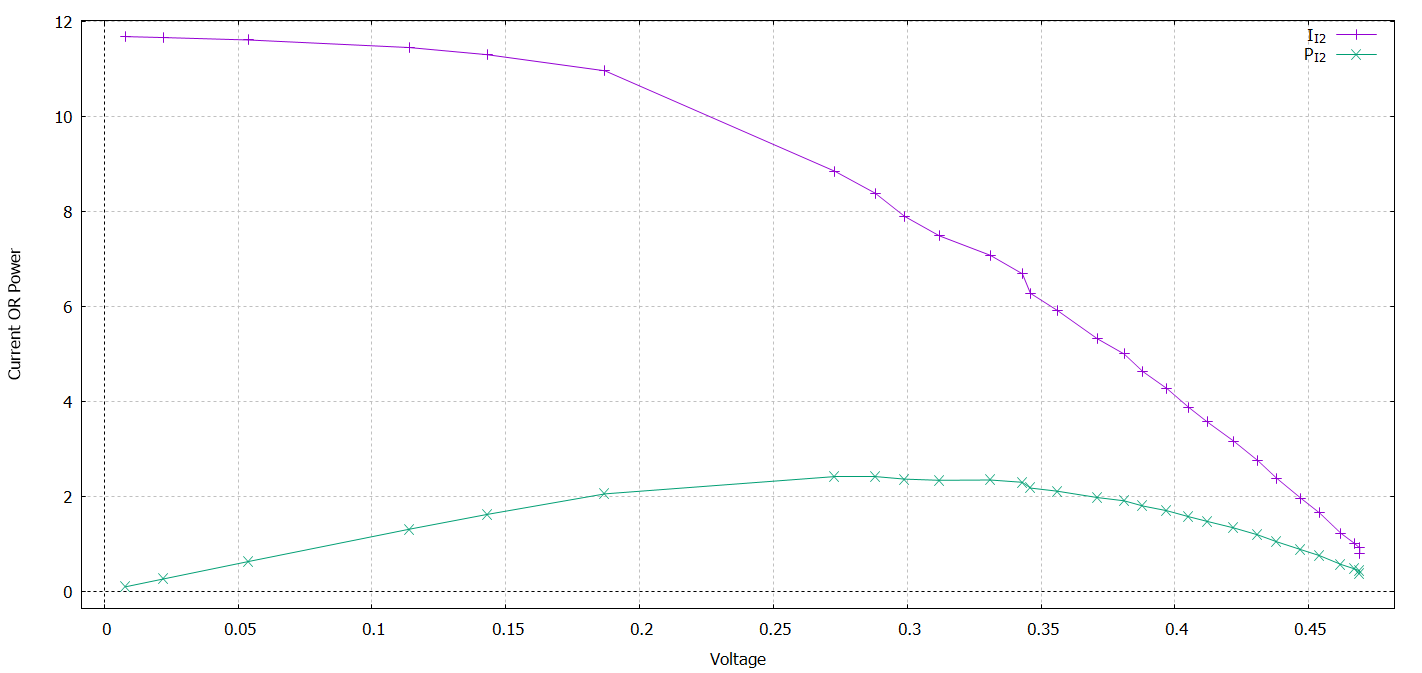
\includegraphics[width = \linewidth, trim = {0 0 0 0}, clip]{Part2_I2.png}
		\caption{Illumination Current I2}
	\end{subfigure} 
	\caption{Part 2 - I-V and P-V Characteristics}
\end{figure}

\begin{center}
 \begin{tabular}{||c c c||c c c||} 
 \hline
 \multicolumn{3}{||c||}{I1} & \multicolumn{3}{|c||}{I2}\\
 \hline
  \( V_L (V) \) & \( I_L (mA) \) & \( P_L (mW) \) & \( V_L (V) \) & \( I_L (mA) \) & \( P_L (mW) \) \\ [0.25ex] 
 \hline
 \hline 
8.80 & 0.008 & 0.07040 & 11.69 & 0.008 & 0.09352 \\ \hline
8.73 & 0.015 & 0.13095 & 11.67 & 0.022 & 0.25674 \\ \hline
8.72 & 0.033 & 0.28776 & 11.62 & 0.054 & 0.62748 \\ \hline
8.69 & 0.062 & 0.53878 & 11.46 & 0.114 & 1.30644 \\ \hline
8.62 & 0.090 & 0.77580 & 11.31 & 0.143 & 1.61733 \\ \hline
8.58 & 0.119 & 1.02102 & 10.97 & 0.187 & 2.05139 \\ \hline
8.49 & 0.144 & 1.22256 & 8.85 & 0.273 & 2.41605 \\ \hline
8.29 & 0.179 & 1.48391 & 8.39 & 0.288 & 2.41632 \\ \hline
7.98 & 0.215 & 1.71570 & 7.90 & 0.299 & 2.36210 \\ \hline
7.72 & 0.245 & 1.89140 & 7.49 & 0.312 & 2.33688 \\ \hline
7.52 & 0.261 & 1.96272 & 7.08 & 0.331 & 2.34348 \\ \hline
7.27 & 0.276 & 2.00652 & 6.69 & 0.343 & 2.29467 \\ \hline
6.98 & 0.290 & 2.02420 & 6.28 & 0.346 & 2.17288 \\ \hline
6.76 & 0.302 & 2.04152 & 5.92 & 0.356 & 2.10752 \\ \hline
6.47 & 0.313 & 2.02511 & 5.32 & 0.371 & 1.97372 \\ \hline
6.13 & 0.326 & 1.99838 & 5.00 & 0.381 & 1.90500 \\ \hline
5.95 & 0.333 & 1.98135 & 4.63 & 0.388 & 1.79644 \\ \hline
5.67 & 0.342 & 1.93914 & 4.27 & 0.397 & 1.69519 \\ \hline
5.35 & 0.352 & 1.88320 & 3.88 & 0.405 & 1.57140 \\ \hline
5.01 & 0.362 & 1.81362 & 3.57 & 0.412 & 1.47084 \\ \hline
4.52 & 0.376 & 1.69952 & 3.16 & 0.422 & 1.33352 \\ \hline
4.18 & 0.385 & 1.60930 & 2.75 & 0.431 & 1.18525 \\ \hline
3.87 & 0.392 & 1.51704 & 2.38 & 0.438 & 1.04244 \\ \hline
3.27 & 0.406 & 1.32762 & 1.96 & 0.447 & 0.87612 \\ \hline
2.91 & 0.415 & 1.20765 & 1.65 & 0.454 & 0.74910 \\ \hline
2.41 & 0.426 & 1.02666 & 1.22 & 0.462 & 0.56364 \\ \hline
2.02 & 0.435 & 0.87870 & 1.01 & 0.467 & 0.47167 \\ \hline
1.53 & 0.445 & 0.68085 & 0.91 & 0.469 & 0.42679 \\ \hline
1.10 & 0.454 & 0.49940 & 0.79 & 0.469 & 0.37051 \\ \hline
0.84 & 0.459 & 0.38556 & - & - & - \\ \hline
0.74 & 0.461 & 0.34114 & - & - & - \\ \hline
\end{tabular}
\end{center}

\subsection{Part 3}

The following table provides the open circuit voltage across the solar panel \( V_{OC} \) and short circuit current \( I_{SC} \) for a given illumination which is given by the current flowing through the LED bank \( I_{LED} \).

\begin{figure}[H]
	\begin{subfigure}[b]{0.6\linewidth}
	   	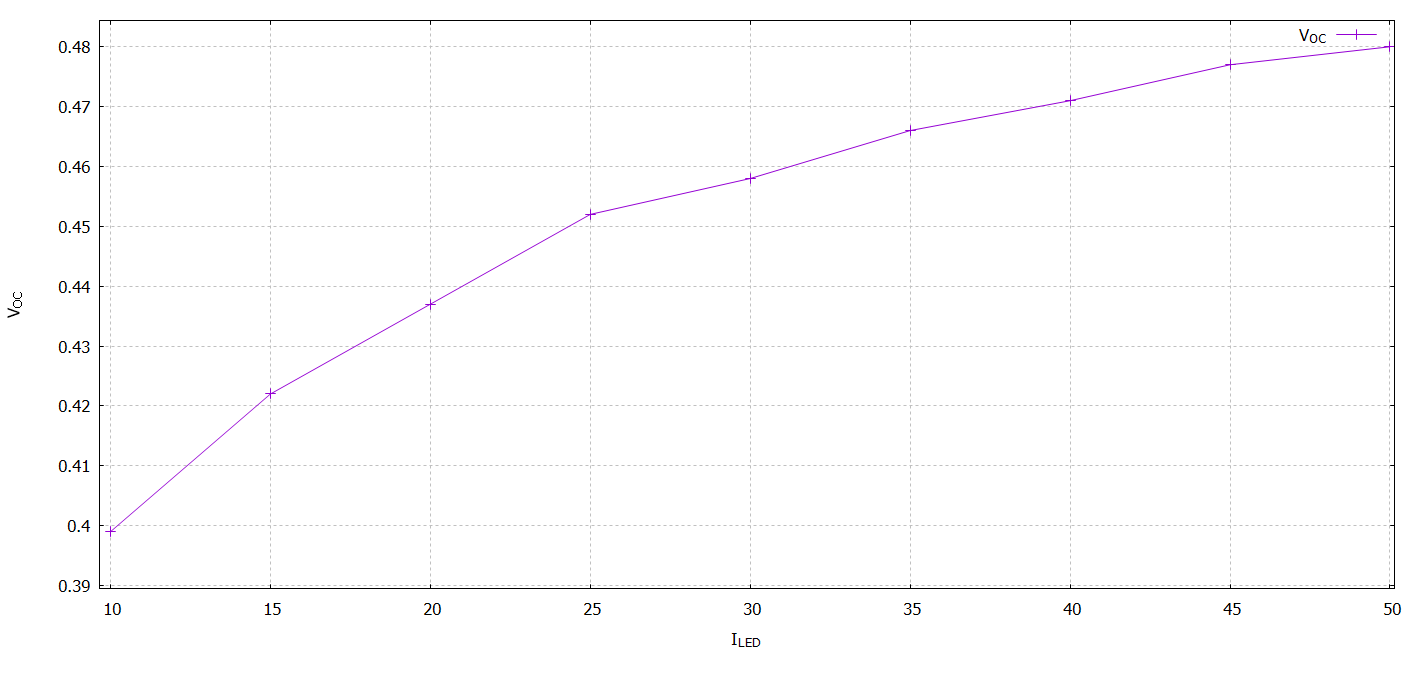
\includegraphics[width = \linewidth, trim = {0 0 0 0}, clip]{Part3_V.png}
		\caption{\( V_{OC}\ vs\ I_{LED} \)}
	\end{subfigure}
	\begin{subfigure}[b]{0.6\linewidth}
		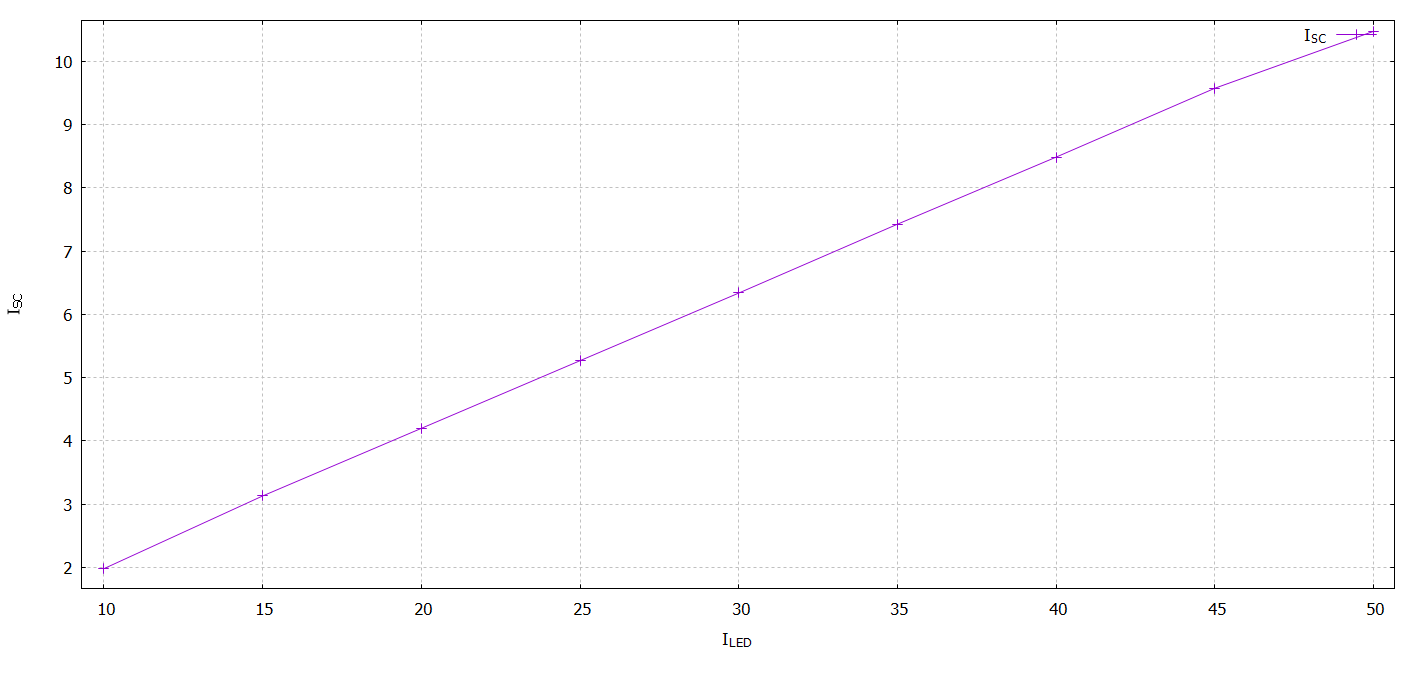
\includegraphics[width = \linewidth, trim = {0 0 0 0}, clip]{Part3_I.png}
		\caption{\( I_{SC}\ vs\ I_{LED} \)}
	\end{subfigure} 
	\caption{Part 3 - Comparison wrt \( I_{LED} \)}
\end{figure}

\begin{center}
 \begin{tabular}{||c c c||} 
 \hline
 \( I_{LED} (mA) \) & \( V_{OC} (V) \) & \( I_{SC} (mA) \) \\ [0.25ex] 
 \hline\hline
 \hline 
10 & 0.399 & 1.98 \\ \hline
15 & 0.422 & 3.13 \\ \hline
20 & 0.437 & 4.20 \\ \hline
25 & 0.452 & 5.27 \\ \hline
30 & 0.458 & 6.34 \\ \hline
35 & 0.466 & 7.43 \\ \hline
40 & 0.471 & 8.49 \\ \hline
45 & 0.477 & 9.58 \\ \hline
50 & 0.480 & 10.48 \\ \hline
\end{tabular}
\end{center}

\section{Simulation}
\begin{verbatim}
 Solar Cell I-V Characteristics

 .include Solar_Cell.txt

 x1 1 0 solar_cell
 vin 2 0 dc 1 ac 0
 r1 2 1 100

 .dc vin -2 2 0.01

 .control
 run

 plot ((v(2)-v(1))/100) vs v(1)

 set hcopydevtype = postscript
 set hcopypscolor = 1
 hardcopy Part1_I1 ((v(2)-v(1))/100) vs v(1)

 .endc
 .end

\end{verbatim}

\begin{figure}[H]
	\begin{subfigure}[b]{0.60\linewidth}
	   	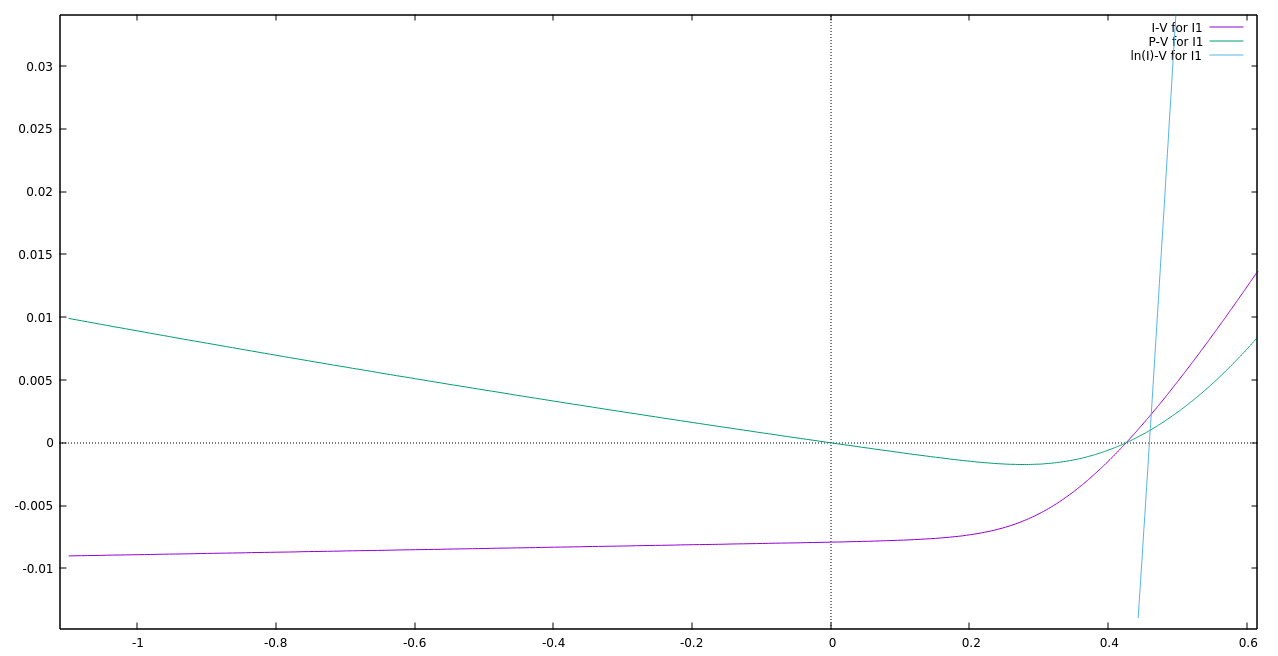
\includegraphics[width = \linewidth, trim = {0 0 0 0}, clip]{part1_I1.png}
		\caption{Illumination Current I1}
	\end{subfigure}
	\begin{subfigure}[b]{0.51\linewidth}
		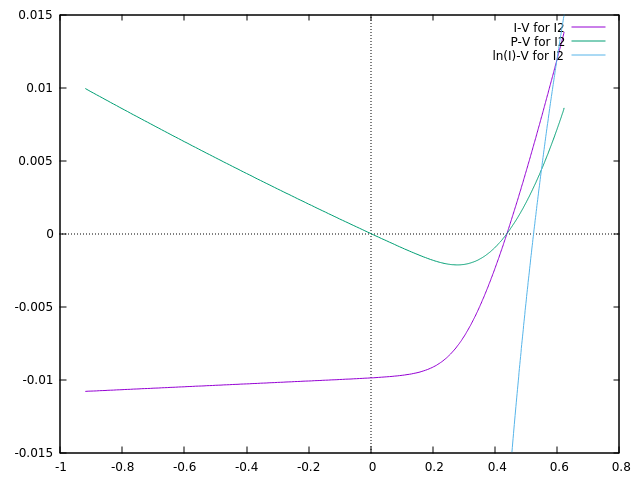
\includegraphics[width = \linewidth, trim = {0 0 0 0}, clip]{part1_I2.png}
		\caption{Illumination Current I2}
	\end{subfigure} 
	\caption{Part 1 - I-V and P-V Characteristics}
\end{figure}

\begin{figure}[H]
\centering
	\begin{subfigure}[b]{0.45\linewidth}
	   	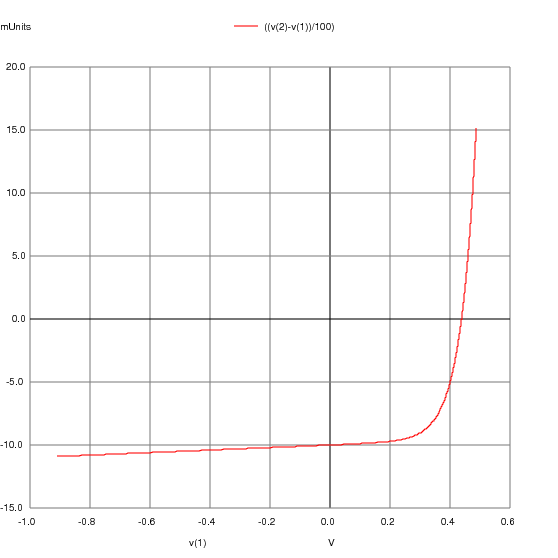
\includegraphics[width = \linewidth, trim = {0 0 0 0}, clip]{part2_rs0.png}
		\caption{\( R_S = 0 \Omega\)}
	\end{subfigure}
	\begin{subfigure}[b]{0.45\linewidth}
		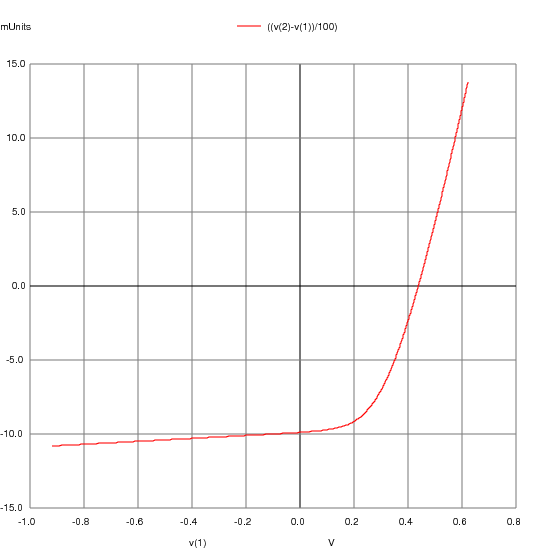
\includegraphics[width = \linewidth, trim = {0 0 0 0}, clip]{part2_rs10.png}
		\caption{\( R_S = 10 \Omega\)}
	\end{subfigure} 
	\begin{subfigure}[b]{0.45\linewidth}
		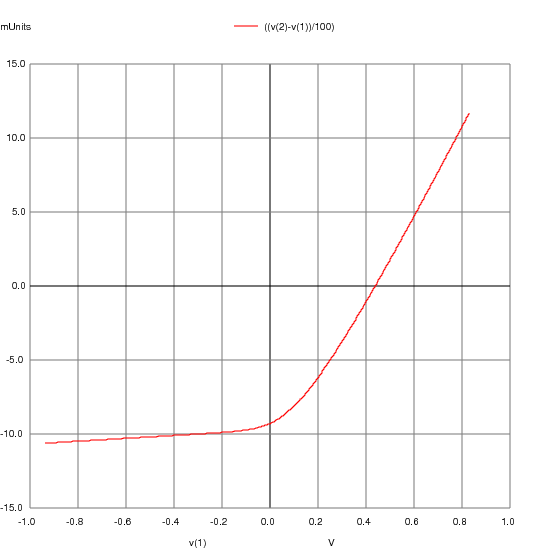
\includegraphics[width = \linewidth, trim = {0 0 0 0}, clip]{part2_rs30.png}
		\caption{\( R_S = 30 \Omega\)}
	\end{subfigure} 
	\caption{Part 2 - Varying the series resistance \( R_S \)}
\end{figure}

\begin{figure}[H]
\centering
	\begin{subfigure}[b]{0.45\linewidth}
		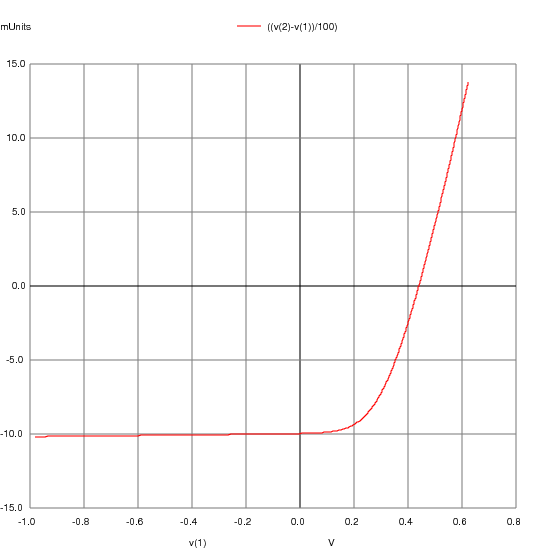
\includegraphics[width = \linewidth, trim = {0 0 0 0}, clip]{part3_rsh5e3.png}
		\caption{\( R_{SH} = 5 \times 10^3 \Omega\)}
	\end{subfigure} 
	\begin{subfigure}[b]{0.45\linewidth}
		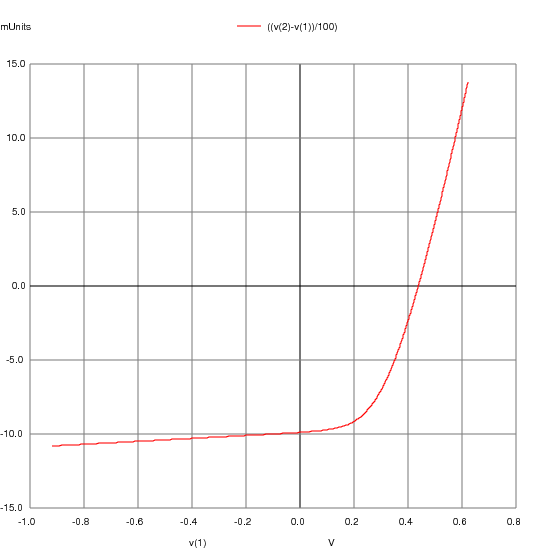
\includegraphics[width = \linewidth, trim = {0 0 0 0}, clip]{part3_rsh1e3.png}
		\caption{\( R_{SH} = 1 \times 10^3 \Omega\)}
	\end{subfigure} 
	\begin{subfigure}[b]{0.45\linewidth}
		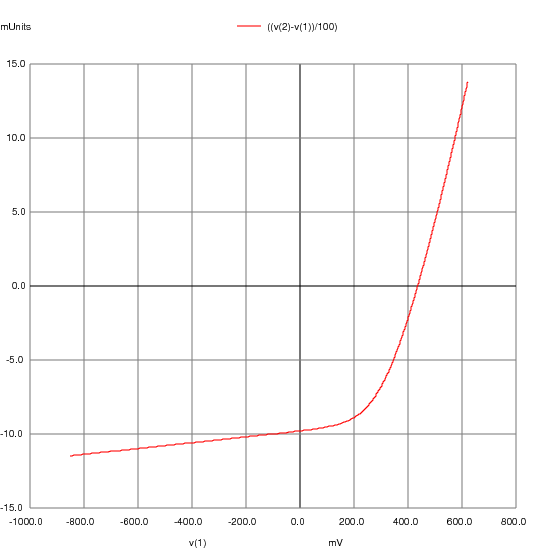
\includegraphics[width = \linewidth, trim = {0 0 0 0}, clip]{part3_rsh5e2.png}
		\caption{\( R_{SH} = 5 \times 10^2 \Omega\)}
	\end{subfigure} 
		\caption{Part 3 - Varying the shunt resistance \( R_{SH} \)}
\end{figure}

\section{Inference from Observations}

\subsection{Part 1}
As expected, when the solar panel is exposed to no light (DARK), the I-V characteristics do not move to the fourth quadrant at all. This implies that power is not generated by the solar panel when no light is irradiated onto it.\\
For an illumination current I1, the current vs voltage graph gives us an equivalent power vs voltage relation which has not been depicted. We realise that the maximum power generated by the solar panel is 2.685 mW for a current of 7.480 mA flowing through it and a given voltage of 0.359 V across it. Since the short-circuit current is 8.840 mA and the open circuit voltage is approximately 0.475 V, we can calculate the fill factor \( FF_{I1} \) as: \[ FF_{I1} = \frac{V_{MP} \times I_{MP}}{V_{OC} \times I_{SC}} = \frac{0.359 \times 7.480}{0.475 \times 8.840} = 0.6395\]
For an illumination current I2 similarly, the current vs voltage graph gives us an equivalent power vs voltage relation which has not been depicted. We realise that the maximum power generated by the solar panel is 3.761 mW for a current of 10.030 mA flowing through it and a given voltage of 0.375 V across it. Since the short-circuit current is 11.740 mA and the open circuit voltage is approximately 0.488 V, we can calculate the fill factor \( FF_{I2} \) as: \[ FF_{I2} = \frac{V_{MP} \times I_{MP}}{V_{OC} \times I_{SC}} = \frac{0.375 \times 10.030}{0.488 \times 11.740} = 0.6565\]

\subsection{Part 2}

The second part measured the current flowing through the resistance and the voltage across the same. Hence both these values were positive when the solar panel was generating power.\\
For an illumination current I1, we observe the required variation in current and power with respect to voltage. The observed current passing through the LED bank, \( I_{LED} = 0.03 mA \). The maximum power generated by the solar panel is 2.0415 mW for a current of 6.7600 mA flowing through it and a given voltage of 0.3020 V across it. Since the short-circuit current is 8.80 mA and the open circuit voltage is approximately 0.474 V, we can calculate the fill factor \( FF_{I1} \) as: \[ FF_{I1} = \frac{V_{MP} \times I_{MP}}{V_{OC} \times I_{SC}} = \frac{0.3020 \times 7.760}{0.474 \times 8.80} = 0.5618\]
For an illumination current I2, we observe the required variation in current and power with respect to voltage. The observed current passing through the LED bank, \( I_{LED} = 0.04 mA \). The maximum power generated by the solar panel is 2.5224 mW for a current of 9.9700 mA flowing through it and a given voltage of 0.2530 V across it. Since the short-circuit current is 11.69 mA and the open circuit voltage is approximately 0.485 V, we can calculate the fill factor \( FF_{I2} \) as: \[ FF_{I2} = \frac{V_{MP} \times I_{MP}}{V_{OC} \times I_{SC}} = \frac{0.2530 \times 9.9700}{0.485 \times 11.69} = 0.4449\]

\subsection{Part 3}

In this part, we notice that \( V_{OC} \) and \( I_{SC} \) acquire a linearly increasing relation with respect to the LED bank current \( I_{LED} \). The part involving \( V_{OC} \) can be explained using the fact that, as irradiation increases, the potential across the depletion region of the p-n junction increases, hence increases the open-circuit voltage \( V_{OC} \) .\\
For a higher irradiation, the potential across the depletion region of the p-n junction increases as mentioned. However the resistance of the solar cell, which arises due to the quasi-neutral non-depletion region, remains more of less constant. This leads to an increase in \( I_{SC} \).

\section{Inference from Simulations}

\subsection{Part 1}

For an illumination current I1, the ideality factor \( \eta \) can be calculated by taking the slope of the log(I)-V graph and using \( \frac{d(log(I))}{dV} = \frac{q}{\eta \times kT} \). We take two points namely (V, I) = (0.461, 2.189) and (0.462, 2.275). Using the following formula, we can obtain the ideality factor: \[ \eta  = \frac{q}{\frac{d(log(I))}{dV} \times kT} = \frac{1.6 \times 10^{-19}}{12.759 \times \left( 25.7 \times 10^{-3} \times 1.6 \times 10^{-19} \right)} = 3.0496 \]
Similarly, for an illumination current I2, we take two points namely (V, I) = (0.473, 2.367) and (0.475, 2.245). Using the following formula, we can obtain the ideality factor: \[ \eta  = \frac{q}{\frac{d(log(I))}{dV} \times kT} = \frac{1.6 \times 10^{-19}}{12.597 \times \left( 25.7 \times 10^{-3} \times 1.6 \times 10^{-19} \right)} = 3.0890 \]
Hence we observe that the ideality factor of the solar cell according to the simulation is approximately 3.\\
For an illumination current I1, the maximum power generated by the solar panel is 1.73 mW for a current of 6.1936 mA flowing through it and a given voltage of 0.2794 V across it. Since the short-circuit current is 8.00 mA and the open circuit voltage is approximately 0.425 V, we can calculate the fill factor \( FF_{I1} \) as: \[ FF_{I1} = \frac{V_{MP} \times I_{MP}}{V_{OC} \times I_{SC}} = \frac{0.2794 \times 6.1936}{0.425 \times 8.00} = 0.5088\]
For an illumination current I2, the maximum power generated by the solar panel is 2.1476 mW for a current of 7.6920 mA flowing through it and a given voltage of 0.279 V across it. Since the short-circuit current is 10.00 mA and the open circuit voltage is approximately 0.438 V, we can calculate the fill factor \( FF_{I2} \) as: \[ FF_{I2} = \frac{V_{MP} \times I_{MP}}{V_{OC} \times I_{SC}} = \frac{0.279 \times 7.6920}{0.438 \times 10.00} = 0.4903\]
There indeed happens to be a discrepancy in the values obtained. We may assume these were due to instrumentation, human and noise errors.

\subsection{Part 2}

The I-V curve in the positive V region tends to resemble that of a resistor with more intensity as the value of \( R_S \) increases. This is quite an expected result since, given the equation of the solar cell as \[ I = I_{D_1} + I_{D_2} - I_{SH} - I_L = I_{0,1}\left[ e^{\frac{qV}{kT}} - 1 \right] + I_{0,2}\left[ e^{\frac{qV}{2kT}} - 1 \right] - \frac{V+I R_s}{R_{SH}} - I_L\] the linear relation between current and voltage caused by \( R_S \) increases as the value of \( R_S \) increases.

\subsection{Part 3}

The I-V curve in the negative V region tends to take a flatter slope as the value of \( R_{SH} \) increases. This is again an expected result since, from the equation of the solar cell, the linear relation between the current and voltage is inversely proportional to the value of \( R_{SH} \). As the value of \( R_{SH} \) increases, the current passing through it decreases, hence reducing effect caused by it.

\end{document}
